\chapter{Recurrent Neural Networks (RNN)} \label{chapter: Recurrent Neural Networks (RNN)}


\begin{figure}[H]
    \centering
    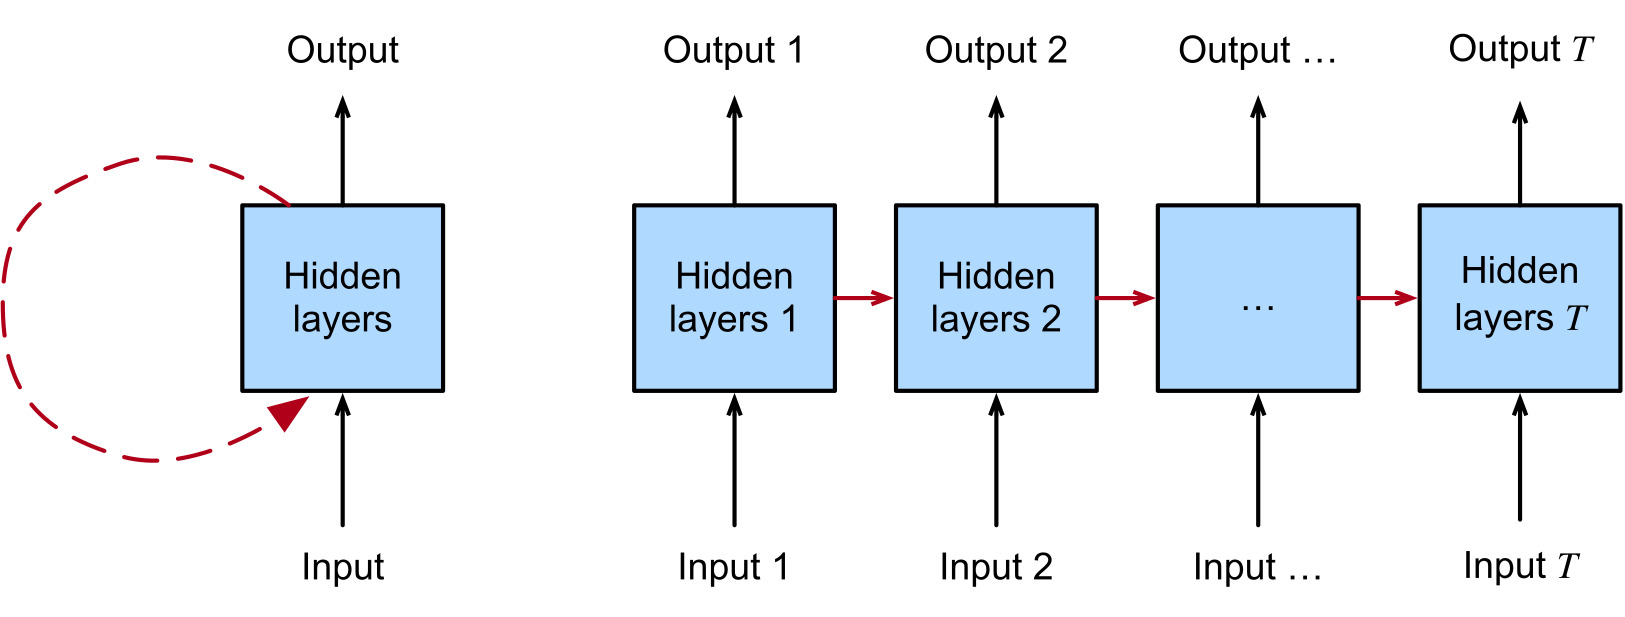
\includegraphics[width=\linewidth, height=3cm, keepaspectratio]{Pictures/Recurrent-Neural-Networks/unfolded-rnn.jpg}
    \caption*{On the left recurrent connections are depicted via cyclic edges. On the right, we unfold the RNN over time steps.}
\end{figure}


\begin{enumerate}
    \item A great many learning tasks require dealing with \textbf{sequential data}. 
    
    \item Image captioning, speech synthesis, and music generation all require that models produce outputs consisting of sequences. 
    
    \item In other domains, such as time series prediction, video analysis, and musical information retrieval, a model must learn from inputs that are sequences. 
    
    \item These demands often arise simultaneously: tasks such as translating passages of text from one natural language to another, engaging in dialogue, or controlling a robot, demand that models both ingest and output sequentially structured data.

    \item Recurrent neural networks (RNNs) are deep learning models that capture the dynamics of sequences via \textbf{recurrent connections}, which can be thought of as \textbf{cycles in the network of nodes}.

    \item It is the feedforward nature of neural networks that makes the order of computation unambiguous. \\
    However, recurrent edges are defined in a precise way that ensures that no such ambiguity can arise.

    \item Recurrent neural networks are \textbf{unrolled} across time steps (or sequence steps), with the same underlying parameters applied at each step. 
    
    \item While the standard connections are applied \textbf{synchronously} to propagate each layer’s activations to the subsequent layer at the same time step, the recurrent connections are \textbf{dynamic}, passing information across adjacent time steps.

    \item RNNs can be thought of as feedforward neural networks where each layer’s parameters (both conventional and recurrent) are shared across time steps.

    \item While the inputs and targets for many fundamental tasks in machine learning cannot easily be represented as fixed-length vectors, they can often nevertheless be represented as varying-length sequences of fixed-length vectors.\\
    \textbf{For example}: documents can be represented as sequences of words; medical records can often be represented as sequences of events (encounters, medications, procedures, lab tests, diagnoses); videos can be represented as varying-length sequences of still images.

    \item 
\end{enumerate}


\section{Working with Sequences \cite{dnn-1}}

\begin{customTableWrapper}{1.5}
\begin{longtable}{l l p{8cm}}
    $\mathbf{x}$ & $\in \mathbb{R}^d$ & single feature vector \\
    $\mathbf{x}_1, \cdots, \mathbf{x}_T$ & $\in \mathbb{R}^d$ & ordered list of feature vectors \\
    $\mathbf{x}_t$ & $\in \mathbb{R}^d$ & each feature vector \\
    $t$ & $\in \mathbb{Z}^+$ & time step \\
\end{longtable}
\end{customTableWrapper}


\begin{enumerate}[itemsep=0.15cm]
    \item Some datasets consist of a single \textbf{massive sequence}\\
    \textbf{For example}, the extremely long streams of sensor readings that might be available to climate scientists.\\
    In such cases, we might create training datasets by randomly sampling subsequences of some predetermined length.

    \item Often data arrives as a \textbf{collection of sequences}\\
    \textbf{Examples}:
    \begin{enumerate}
        \item a collection of documents, each represented as its own sequence of words, and each having its own length $T_i$
        
        \item sequence representation of patient stays in the hospital, where each stay consists of a number of events and the sequence length depends roughly on the length of the stay.
        
    \end{enumerate}

    \item we \textbf{CANNOT} assume that the data arriving at each time step are independent of each other.\\
    \textbf{For example}, the words that likely to appear later in a document depend heavily on words occurring earlier in the document.\\
    The medicine a patient is likely to receive on the 10th day of a hospital visit depends heavily on what transpired in the previous nine days.

    \item we require only that the sequences themselves are sampled from some fixed underlying distribution over entire sequences

    \item sequence-to-sequence tasks take two forms: 
    \begin{enumerate}
        \item \textbf{aligned}: where the input at each time step aligns with a corresponding target (e.g., part of speech tagging); 
        
        \item \textbf{unaligned}: where the input and target do not necessarily exhibit a step-for-step correspondence (e.g., machine translation).
    \end{enumerate}

    \item we can tackle the most straightforward problem: unsupervised density modeling (also called sequence modeling). Here, given a collection of sequences, our goal is to estimate the probability mass function that tells us how likely we are to see any given sequence, i.e., $p(\mathbf{x}_1, \ldots, \mathbf{x}_T)$

\end{enumerate}


\section{Autoregressive Models \cite{dnn-1}} \label{Autoregressive Models}

\begin{customTableWrapper}{1.5}
\begin{table}[H]
    \centering
    \begin{tabular}{l p{8cm}}
        $P(x_t \mid x_{t-1}, \ldots, x_1)$ & probability distribution \\
        $\mathbb{E}[(x_t \mid x_{t-1}, \ldots, x_1)]$ & conditional expectation \\
    \end{tabular}
\end{table}
\end{customTableWrapper}

\begin{enumerate}
    \item At each time step $t$, we observe the input, $x_t$, of the index at that time.

    \item models that regress the value of a signal on the previous values of that same signal are naturally called \textbf{autoregressive models}.

    \item There is just one major problem: the number of inputs, $x_{t-1}, \cdots, x_1$ varies, depending on $t$.\\
    In other words, the number of inputs increases with the amount of data that we encounter. \\
    Thus if we want to treat our historical data as a training set, we are left with the problem that each example has a different number of features.

    \item we might believe that although long sequences $x_{t-1}, \ldots, x_1$ are available, it may not be necessary to look back so far in the history when predicting the near future.\\
    In this case we might content ourselves to condition on some window of length $\tau$ and only use $x_{t-1}, \ldots, x_{t-\tau}$ observations.\\
    The immediate benefit is that now the number of arguments is always the same, at least for $t > \tau$.\\
    This allows us to train any linear model or deep network that requires fixed-length vectors as inputs.

    \item we might develop models that maintain some summary $h_t$ of the past observations and at the same time update $h_t$ in addition to the prediction $\hat{x}_t$.\\
    This leads to models that estimate not only $x_t$ with $\hat{x}_t = P(x_t \mid h_{t})$ but also updates of the form $h_t = g(h_{t-1}, x_{t-1})$. \\
    Since $h_t$ is never observed, these models are also called \textbf{latent autoregressive models}\indexlabel{latent autoregressive models}.

    \item To construct training data from historical data, one typically creates examples by sampling windows randomly.

    \item we often assume that while the specific values of $x_t$ might change, the dynamics according to which each subsequent observation is generated given the previous observations do not. Statisticians call dynamics that do not change \textbf{stationary}.
    
\end{enumerate}




\section{Sequence Models \cite{dnn-1}} \label{Sequence Models}

\begin{enumerate}
    \item especially when working with language, we wish to estimate the joint probability of an entire sequence\\
    Generally, these estimated functions are called sequence models and for natural language data, they are called language models.

    \item The field of sequence modeling has been driven so much by natural language processing, that we often describe sequence models as “language models”, even when dealing with non-language data.

    \item language modeling gives us not only the capacity to evaluate likelihood, but the ability to sample sequences, and even to optimize for the most likely sequences.

    \item While language modeling might not, at first glance, look like an autoregressive problem, we can reduce language modeling to autoregressive prediction by decomposing the joint density of a sequence $p(x_1, \ldots, x_T)$ into the product of conditional densities in a left-to-right fashion by applying the chain rule of probability:
    \[
        \hfill
        P(x_1, \cdots, x_T) = P(x_1) \dprod_{t=2}^T P(x_t \mid x_{t-1}, \cdots, x_1)
        \hfill
    \]

    \item If we are working with discrete signals such as words, then the autoregressive model must be a probabilistic classifier, outputting a full probability distribution over the vocabulary for whatever word will come next, given the leftwards context.

\end{enumerate}


\section{Markov Models \cite{dnn-1}}\label{rnn: Markov Models}

\begin{enumerate}
    \item we condition only on the $\tau$ previous time steps, i.e., $x_{t-1}, \ldots, x_{t-\tau}$, rather than the entire sequence history $x_{t-1}, \ldots, x_1$.
    
    \item Whenever we can throw away the history beyond the previous $\tau$ steps without any loss in predictive power, we say that the sequence satisfies a \textbf{Markov condition}\indexlabel{Markov condition}, i.e., that \textit{the future is conditionally independent of the past, given the recent history}. 
    
    \item When $\tau = 1$, we say that the data is characterized by a \textbf{first-order Markov model}\indexlabel{first-order Markov model}, and when $\tau = k$, we say that the data is characterized by a $k^{\textrm{th}}$-order Markov model.
    
    \item For when the first-order Markov condition holds ($\tau = 1$) the factorization of our joint probability becomes a product of probabilities of each word given the previous word:
    \[
        \hfill
        P(x_1, \ldots, x_T) = P(x_1) \prod_{t=2}^T P(x_t \mid x_{t-1})
        \hfill
    \]

    \item we compromise, obviating computational and statistical difficulties by training models whose validity depends on a $k^{\textrm{th}}$-order Markov condition.

    \item With discrete data, a true Markov model simply counts the number of times that each word has occurred in each context, producing the relative frequency estimate of $P(x_t \mid x_{t-1})$.\\
    Whenever the data assumes only discrete values (as in language), the most likely sequence of words can be computed efficiently using \textbf{dynamic programming}.

\end{enumerate}

\subsection{Order of Decoding \cite{dnn-1}}

\begin{enumerate}[itemsep=0.15cm]
    \item the factorization of a text sequence $P(x_1, \ldots, x_T)$ as a \textbf{left-to-right} chain of conditional probabilities and not right-to-left or some other, seemingly random order.
    \[
        \hfill
        P(x_1, \ldots, x_T) = P(x_T) \prod_{t=T-1}^1 P(x_t \mid x_{t+1}, \ldots, x_T)
        \hfill
    \]

    \item there is nothing wrong with unfolding in reverse order.\\
    However, there are many reasons why factorizing text in the same direction in which we read it (left-to-right for most languages, but right-to-left for Arabic and Hebrew) is preferred for the task of language modeling.

    \item this is just a more natural direction for us to think about\\
    ability to anticipate which words and phrases are likely to come next\\
    even if we had no other reason to prefer such in-order decodings, they would be useful if only because we have better intuitions for what should be likely when predicting in this order.

    \item by factorizing in order, we can assign probabilities to arbitrarily long sequences using the same language model.\\
    To convert a probability over steps $1$ through $t$ into one that extends to word $t+1$ we simply multiply by the conditional probability of the additional token given the previous ones: 
    \[
        \hfill
        P(x_{t+1}, \ldots, x_1) = P(x_{t}, \ldots, x_1) \cdot P(x_{t+1} \mid x_{t}, \ldots, x_1)
        \hfill
    \]

    \item we have stronger predictive models for predicting adjacent words than words at arbitrary other locations. \\
    While all orders of factorization are valid, they do not necessarily all represent equally easy predictive modeling problems.\\
    we believe that future events cannot influence the past. Hence, if we change $x_t$, we may be able to influence what happens for $x_{t+1}$ going forward but not the converse.\\
    That is, if we change $x_t$, the distribution over past events will not change.\\
    In some contexts, this makes it easier to predict $P(x_{t+1} \mid x_t)$ than to predict $P(x_t \mid x_{t+1})$\\
    we can find $x_{t+1} = f(x_t) + \epsilon$ for some additive noise $\epsilon$, whereas the converse is not true

    
\end{enumerate}




\section{Language Models \cite{dnn-1}} \label{Language Models}

SEE: \fullref{Sequence Models}

\begin{enumerate}
    \item Assume that the tokens in a text sequence of length $T$ are in turn $x_1, x_2, \cdots, x_T$

    \item The goal of language models is to estimate the joint probability of the whole sequence: $P(x_1, x_2, \ldots, x_T)$ 

    \item an ideal language model should generate natural text on its own, simply by drawing one token at a time $x_t \sim P(x_t \mid x_{t-1}, \ldots, x_1)$

    \item Quite unlike the monkey using a typewriter, all text emerging from such a model would pass as natural language, e.g., English text

    \item it would be sufficient for generating a meaningful dialog, simply by conditioning the text on previous dialog fragments.

    
\end{enumerate}


\subsection{Converting Raw Text into Sequence Data \cite{dnn-1}}

\begin{enumerate}
    \item we will need some basic tools for converting raw text into sequences of the appropriate form.

    \item Typical preprocessing pipelines execute the following steps:
    \begin{enumerate}
        \item Load text as strings into memory.

        \item Split the strings into tokens (e.g., words or characters).

        \item Build a vocabulary dictionary to associate each vocabulary element with a numerical index.

        \item Convert the text into sequences of numerical indices.

    \end{enumerate}
\end{enumerate}


\subsubsection{Tokenization \cite{dnn-1}}

\begin{enumerate}
    \item Tokens are the atomic (indivisible) units of text. Each time step corresponds to 1 token, but what precisely constitutes a token is a design choice. 
    
    \item \textbf{For example}, we could represent the sentence “Baby needs a new pair of shoes” as a sequence of 7 words, where the set of all words comprise a large vocabulary (typically tens or hundreds of thousands of words).\\
    Or we would represent the same sentence as a much longer sequence of 30 characters, using a much smaller vocabulary (there are only 256 distinct ASCII characters).

    \item These tokens are still strings.

\end{enumerate}

\subsubsection{Vocabulary \cite{dnn-1}}

\begin{enumerate}
    \item the inputs to our models must ultimately consist of numerical inputs

    \item we determine the set of \textbf{unique tokens} in our training corpus. 
    
    \item We then assign a \textbf{numerical index} to each unique token. 
    
    \item \textbf{Rare vocabulary elements} are often \textbf{dropped} for convenience. 
    
    \item Whenever we encounter a token at training or test time that had not been previously seen or was dropped from the vocabulary, we represent it by a special “\verb|<unk>|” token, signifying that this is an \textbf{unknown value}.

    \item Note that we have not lost any information and can easily convert our dataset back to its original (string) representation.

\end{enumerate}

















